% Generated by make_figure.py - do not edit by hand.
\begin{figure}[!ht]
\centering
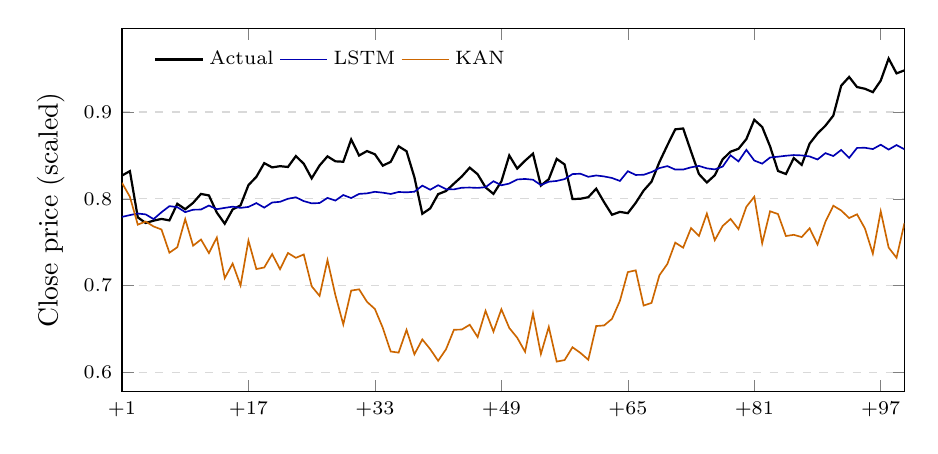
\begin{tikzpicture}
\begin{axis}[
  width=0.95\textwidth, height=6.2cm,
  xmin=0, xmax=99, ylabel={Close price (scaled)},
  xtick={0,16,32,48,64,80,96},
  xticklabels={+1,+17,+33,+49,+65,+81,+97},
  x tick label style={font=\scriptsize},
  y tick label style={font=\scriptsize},
  legend style={font=\scriptsize, draw=none}, legend pos=north west,
  legend columns=3, ymajorgrids, grid style={dashed,gray!30}]
\addplot+[mark=none, thick, black] coordinates {
(0,0.8268) (1,0.8319) (2,0.7787) (3,0.7722) (4,0.7749) (5,0.7769) (6,0.7752) (7,0.7943) (8,0.7881) (9,0.7954) (10,0.8057) (11,0.8039) (12,0.7842) (13,0.7714) (14,0.7878) (15,0.7925) (16,0.8158) (17,0.8253) (18,0.8411) (19,0.8362) (20,0.8376) (21,0.8367) (22,0.8492) (23,0.8404) (24,0.8236) (25,0.8384) (26,0.8489) (27,0.8432) (28,0.8427) (29,0.8684) (30,0.8499) (31,0.8550) (32,0.8513) (33,0.8382) (34,0.8426) (35,0.8605) (36,0.8548) (37,0.8248) (38,0.7828) (39,0.7890) (40,0.8054) (41,0.8090) (42,0.8175) (43,0.8258) (44,0.8359) (45,0.8283) (46,0.8132) (47,0.8057) (48,0.8200) (49,0.8499) (50,0.8349) (51,0.8439) (52,0.8520) (53,0.8153) (54,0.8226) (55,0.8460) (56,0.8396) (57,0.7998) (58,0.8001) (59,0.8019) (60,0.8117) (61,0.7961) (62,0.7817) (63,0.7850) (64,0.7835) (65,0.7954) (66,0.8095) (67,0.8198) (68,0.8424) (69,0.8616) (70,0.8800) (71,0.8810) (72,0.8545) (73,0.8285) (74,0.8188) (75,0.8271) (76,0.8455) (77,0.8543) (78,0.8576) (79,0.8688) (80,0.8910) (81,0.8827) (82,0.8603) (83,0.8321) (84,0.8286) (85,0.8469) (86,0.8391) (87,0.8635) (88,0.8752) (89,0.8842) (90,0.8958) (91,0.9303) (92,0.9403) (93,0.9287) (94,0.9267) (95,0.9228) (96,0.9361) (97,0.9615) (98,0.9444) (99,0.9479)};
\addplot+[mark=none, semithick, blue!70!black] coordinates {
(0,0.7792) (1,0.7813) (2,0.7831) (3,0.7821) (4,0.7767) (5,0.7846) (6,0.7916) (7,0.7905) (8,0.7847) (9,0.7875) (10,0.7877) (11,0.7923) (12,0.7881) (13,0.7896) (14,0.7910) (15,0.7896) (16,0.7907) (17,0.7951) (18,0.7899) (19,0.7958) (20,0.7966) (21,0.8001) (22,0.8018) (23,0.7974) (24,0.7948) (25,0.7952) (26,0.8011) (27,0.7980) (28,0.8044) (29,0.8009) (30,0.8057) (31,0.8063) (32,0.8081) (33,0.8071) (34,0.8056) (35,0.8079) (36,0.8075) (37,0.8082) (38,0.8152) (39,0.8105) (40,0.8157) (41,0.8111) (42,0.8109) (43,0.8128) (44,0.8130) (45,0.8126) (46,0.8134) (47,0.8203) (48,0.8156) (49,0.8176) (50,0.8223) (51,0.8229) (52,0.8220) (53,0.8159) (54,0.8197) (55,0.8206) (56,0.8227) (57,0.8285) (58,0.8289) (59,0.8254) (60,0.8269) (61,0.8258) (62,0.8240) (63,0.8206) (64,0.8318) (65,0.8275) (66,0.8277) (67,0.8308) (68,0.8354) (69,0.8377) (70,0.8337) (71,0.8337) (72,0.8363) (73,0.8379) (74,0.8351) (75,0.8339) (76,0.8371) (77,0.8501) (78,0.8431) (79,0.8564) (80,0.8441) (81,0.8405) (82,0.8476) (83,0.8485) (84,0.8496) (85,0.8504) (86,0.8500) (87,0.8488) (88,0.8453) (89,0.8526) (90,0.8493) (91,0.8563) (92,0.8471) (93,0.8586) (94,0.8588) (95,0.8573) (96,0.8623) (97,0.8567) (98,0.8619) (99,0.8570)};
\addplot+[mark=none, semithick, orange!80!black] coordinates {
(0,0.8184) (1,0.8024) (2,0.7703) (3,0.7739) (4,0.7682) (5,0.7647) (6,0.7380) (7,0.7443) (8,0.7767) (9,0.7461) (10,0.7532) (11,0.7376) (12,0.7555) (13,0.7087) (14,0.7255) (15,0.7003) (16,0.7520) (17,0.7192) (18,0.7210) (19,0.7364) (20,0.7190) (21,0.7377) (22,0.7321) (23,0.7360) (24,0.6994) (25,0.6883) (26,0.7295) (27,0.6892) (28,0.6555) (29,0.6944) (30,0.6959) (31,0.6815) (32,0.6732) (33,0.6515) (34,0.6243) (35,0.6230) (36,0.6492) (37,0.6211) (38,0.6382) (39,0.6270) (40,0.6136) (41,0.6269) (42,0.6493) (43,0.6496) (44,0.6551) (45,0.6409) (46,0.6711) (47,0.6472) (48,0.6729) (49,0.6514) (50,0.6402) (51,0.6240) (52,0.6682) (53,0.6214) (54,0.6526) (55,0.6127) (56,0.6144) (57,0.6292) (58,0.6227) (59,0.6148) (60,0.6536) (61,0.6543) (62,0.6619) (63,0.6826) (64,0.7157) (65,0.7177) (66,0.6772) (67,0.6802) (68,0.7121) (69,0.7250) (70,0.7496) (71,0.7438) (72,0.7663) (73,0.7573) (74,0.7830) (75,0.7524) (76,0.7688) (77,0.7769) (78,0.7652) (79,0.7909) (80,0.8024) (81,0.7488) (82,0.7857) (83,0.7825) (84,0.7572) (85,0.7586) (86,0.7560) (87,0.7661) (88,0.7475) (89,0.7736) (90,0.7921) (91,0.7866) (92,0.7779) (93,0.7822) (94,0.7659) (95,0.7369) (96,0.7856) (97,0.7439) (98,0.7322) (99,0.7720)};
\legend{Actual, LSTM, KAN}
\end{axis}
\end{tikzpicture}
\caption{TODO write caption}
\label{fig:figure_h100_traj-1_s0_pykan}
\end{figure}
